\documentclass[10pt]{article}

\usepackage{pablo}
\usepackage{yhmath}
\usetikzlibrary{3d,calc}

\usepackage[a5paper,margin=1.4cm]{geometry}

\pagestyle{empty}
\begin{document}

\begin{center}
  \textsc{DM}

  {
    \Large
    Géométrie dans l'espace --- Correction

    \hrule
  }
\end{center}

\begin{exercice}[Perspective cavalière]
  On considère le triangle suivant, avec les longueurs $BC=13cm$, $AC=15cm$, $AH=3cm$.

  \begin{center}
  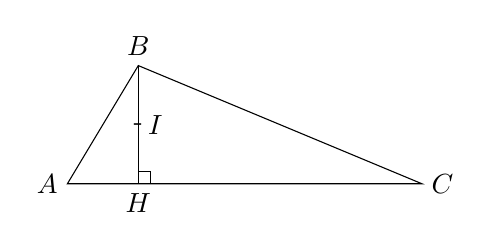
\begin{tikzpicture}[scale=0.3]
    \draw (0,0) node[left]{$A$}-- (3,5) node[above]{$B$} -- (15,0) node[right]{$C$} -- cycle;
    \draw (3,0) node[below]{$H$} -- (3,5) node[midway,right]{$I$} node[midway]{-};
    \draw (3,0.5) -- ++(0.5,0) -- ++(0,-0.5);
  \end{tikzpicture}
\end{center}

  \begin{enumerate}
    \item \emph{Montrer que $BH=5cm$.} Le triangle $BHC$ étant rectangle en $H$, on applique le théorème de Pythagore : $BC^2=HC^2+BH^2$, donc $13^2=12^2+BH^2$. Ainsi, $BH^2=13^2-12^2=169-144=25$. Donc $BH=\sqrt{25}=5$.
    \item \emph{Dessiner en perspective cavalière la pyramide de base $ABC$, de hauteur $7cm$, le sommet de la pyramide étant à la verticale du point $I$ milieu de $BH$. On prendra 30\up{o} comme angle des fuyantes, et 0,8 comme coefficient de réduction.}
  \end{enumerate}
\end{exercice}

Il est possible de dessiner cette pyramide de plusieurs manières différentes, selon que la face $ABC$ est « à l'horizontale » ou « face à nous » (on peut aussi imaginer de placer la pyramide « la tête en bas », par exemple).

\paragraph{Première version : La face $ABC$ est face à nous.} Le triangle $ABC$ étant dessiné en vrai grandeur, on trace la hauteur $[IS]$ de la pyramide : elle passe par le point $I$ milieu de $[BH]$, et elle est perpendiculaire au plan de la feuille : c'est une fuyante. Il faut donc la dessiner avec un angle de 30\up{o} par rapport à l'horizontale, et un coefficient de réduction de 0,8 : sa longueur apparente sera $0,8\times7=5,6\text{~cm}$. Cela donne :

\begin{center}
  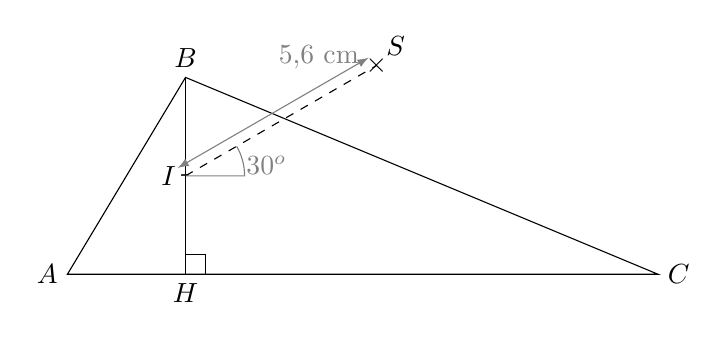
\begin{tikzpicture}[scale=0.5]
    \draw (0,0) node[left]{$A$}-- (3,5) node[above]{$B$} -- (15,0) node[right]{$C$} -- cycle;
    \draw (3,0) node[below]{$H$} -- (3,5) node[midway,left]{$I$} node[midway]{-};
    \draw (3,0.5) -- ++(0.5,0) -- ++(0,-0.5);
    \draw[dashed] (3,2.5) -- ++(30:5.6);
    \coordinate (S) at ($(3,2.5) + (30:5.6)$);
    \draw[gray,latex-latex] ($(3,2.5) + (-0.2,+0.2)$) -- ++(30:5.6) node[left]{5,6~cm};
    \draw (S) node{$\times$} node[above right]{$S$};
    \draw[gray] (3,2.5) -- ++ (1.5,0) arc (0:30:1.5) node[below right]{$30^o$};
  \end{tikzpicture}
\end{center}

Il ne reste qu'à relier le sommet $S$ de la pyramide aux sommets de la base, en mettant en pointillé les arêtes masquées.

\begin{center}
  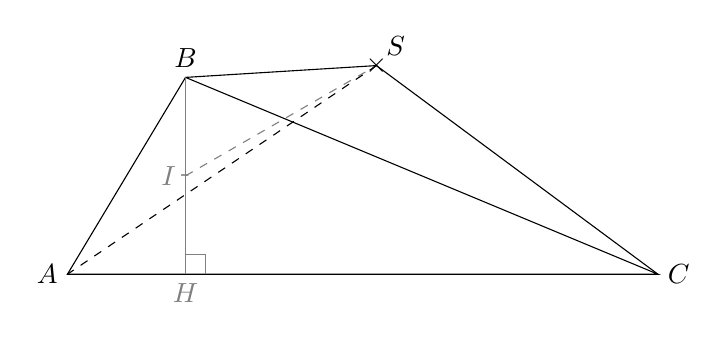
\begin{tikzpicture}[scale=0.5]
    \draw (0,0) node[left]{$A$}-- (3,5) node[above]{$B$} -- (15,0) node[right]{$C$} -- cycle;
    \draw[gray] (3,0) node[below]{$H$} -- (3,5) node[midway,left]{$I$} node[midway]{-};
    \draw[gray] (3,0.5) -- ++(0.5,0) -- ++(0,-0.5);
    \draw[gray,dashed] (3,2.5) -- ++(30:5.6);
    \coordinate (S) at ($(3,2.5) + (30:5.6)$);
    \draw (S) node{$\times$} node[above right]{$S$};
    \draw[dashed] (S) -- (0,0);
    \draw (S) -- (3,5);
    \draw (S) -- (15,0);
  \end{tikzpicture}
\end{center}

  \paragraph{Seconde version : La face $ABC$ est « à l'horizontale »}
  On commence par tracer le segment $[AC]$, en vraie grandeur. Puis on trace la hauteur $[BH]$. C'est une fuyante, donc elle apparait avec un angle de trente degrés et un coefficient de réduction : sa longueur apparente est $5\times0,8=4\text{~cm}$.

  \begin{center}
  \begin{tikzpicture}[scale=0.5]
    \coordinate (A) at (0,0);
    \coordinate (C) at ($(A) + (15,0)$);
    \coordinate (H) at ($(A) + (3,0)$);
    \coordinate (B) at ($(H) + (30:0.8*5)$);

    \draw (A) node[left]{$A$} -- (C) node[right]{$C$};
    \draw[dashed] (H) node[below]{$H$} -- (B) node[right]{$B$};
    \draw[gray,latex-latex] ($(H) + (-0.2,+0.2)$) -- ($(B) + (-0.2,0.2)$) node[midway,above left]{4~cm};
    \draw[gray] ($(H) + (1.5,0)$) arc (0:30:1.5);
    \draw[gray] ($(H) + (1.5,0.5)$) node[right]{$30^o$};
  \end{tikzpicture}
\end{center}

  On peut maintenant finir de tracer le triangle, en traçant les côtés $[AB]$ et $[BC]$, et on place le point $I$, milieu de $[BH]$.

  \begin{center}
  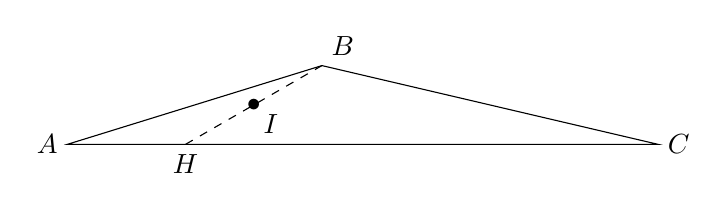
\begin{tikzpicture}[scale=0.5]
    \coordinate (A) at (0,0);
    \coordinate (C) at ($(A) + (15,0)$);
    \coordinate (H) at ($(A) + (3,0)$);
    \coordinate (B) at ($(H) + (30:0.8*5)$);
    \coordinate (I) at ($0.5*(H) + 0.5*(B)$);

    \draw (A) node[left]{$A$} -- (C) node[right]{$C$} -- (B) -- cycle;
    \draw[dashed] (H) node[below]{$H$} -- (B) node[above right]{$B$};
    \draw (I) node{$\bullet$} node[below right]{$I$};
  \end{tikzpicture}
\end{center}

La hauteur $[SI]$ de la pyramide étant dans un plan parallèle à la feuille, elle est dessinée en vraie grandeur. C'est un segment vertical passant par $I$.

  \begin{center}
  \begin{tikzpicture}[scale=0.5]
    \coordinate (A) at (0,0);
    \coordinate (C) at ($(A) + (15,0)$);
    \coordinate (H) at ($(A) + (3,0)$);
    \coordinate (B) at ($(H) + (30:0.8*5)$);
    \coordinate (I) at ($0.5*(H) + 0.5*(B)$);
    \coordinate (S) at ($(I) + (0,7)$);

    \draw (A) node[left]{$A$} -- (C) node[right]{$C$} -- (B) -- cycle;
    \draw[dashed] (H) node[below]{$H$} -- (B) node[above right]{$B$};
    \draw (I) node[below right]{$I$};

    \draw (I) -- (S) node[above]{$S$};
    \draw (I) -- ++(0,0.5) -- ++(30:0.5) -- ++(0,-0.5);
  \end{tikzpicture}
\end{center}

  Il ne reste plus qu'à relier le sommet à chacun des trois points de la base $A$, $B$ et $C$, en traçant en pointillé les arêtes masquées.

  \begin{center}
  \begin{tikzpicture}[scale=0.5]
    \coordinate (A) at (0,0);
    \coordinate (C) at ($(A) + (15,0)$);
    \coordinate (H) at ($(A) + (3,0)$);
    \coordinate (B) at ($(H) + (30:0.8*5)$);
    \coordinate (I) at ($0.5*(H) + 0.5*(B)$);
    \coordinate (S) at ($(I) + (0,7)$);

    \draw (A) node[left]{$A$} -- (C) node[right]{$C$};
    \draw[dashed] (C) -- (B) -- (A);
    \draw[dashed] (H) node[below]{$H$} -- (B) node[above right]{$B$};
    \draw (I) node[below right]{$I$};

    \draw[dashed] (I) -- (S) node[above]{$S$};
    \draw (I) -- ++(0,0.5) -- ++(30:0.5) -- ++(0,-0.5);

    \draw (A) -- (S);
    \draw[dashed] (B) -- (S);
    \draw (C) -- (S);
  \end{tikzpicture}
\end{center}

\begin{exercice}[Surface d'un cône]~

  \begin{center}
    \hspace{\stretch{1}}
  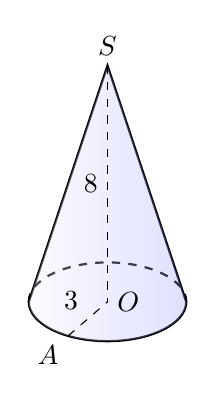
\begin{tikzpicture}
    \draw[thick] (-1,0) arc (180:360:1cm and 0.5cm) -- (0,3) -- cycle;
    \draw[thick,dashed] (-1,0) arc (180:0:1cm and 0.5cm);
    \shade[thick,left color=blue!5!white,right color=blue!40!white,opacity=0.3] (-1,0) arc (180:360:1cm and 0.5cm) -- (0,3) -- cycle;
    \draw[dashed] (240:1cm and 0.5cm) -- (0,0) node[midway,above left]{$3$};
    \draw[dashed] (0,3) -- (0,0) node[midway,left]{$8$};
    \draw (0,0) node[right]{$O$};
    \draw (0,3) node[above]{$S$};
    \draw (240:1cm and 0.5cm) node[below left]{$A$};
  \end{tikzpicture}
    \hspace{\stretch{1}}
  \begin{tikzpicture}[scale=0.3]
    \draw (0,0) circle (3);
    \draw (0,{3+sqrt(73)}) node[above]{$O$} -- ++({-sqrt(73)*sin((1080/sqrt(73))/2)},{-sqrt(73)*cos((1080/sqrt(73))/2)}) node[left]{$B$} arc ({(540-(1080/sqrt(73)))/2}:{(540+(1080/sqrt(73)))/2}:{sqrt(73)}) node[right]{$C$}-- cycle;
    \draw[draw=none] (0,{3+sqrt(73)}) -- ++({-sqrt(73)*sin((1080/sqrt(73))/2)},{-sqrt(73)*cos((1080/sqrt(73))/2)}) node[midway,above]{$R$};
    \draw[dashed] (0,0) -- ++(33:3) node[midway,below]{$3$};
    \draw ({-2*sin((1080/sqrt(73))/2)},{3+sqrt(73)-2*cos((1080/sqrt(73))/2)}) arc ({(540-(1080/sqrt(73)))/2}:{(540+(1080/sqrt(73)))/2}:{2});
    \draw (0,{3+sqrt(73)-2}) node[below]{$\alpha$};
  \end{tikzpicture}
    \hspace{\stretch{1}}
    ~
  \end{center}

  On considère un cône de révolution, dont la base est un cercle de rayon 3~cm, et de hauteur 8~cm. Le but de l'exercice est de déterminer l'aire de ce solide, dont le patron est donné à droite.

  Dans la suite de l'exercice, toutes les longueurs considérées sont en centimètres.

  \begin{enumerate}
    \item \emph{On considère le triangle $OAS$. Quelle est sa nature ? Lire sur le dessin les longueurs des segments $[AO]$ et $[OS]$. En déduire que $SA=\sqrt{73}$.} Le triangle $OAS$ est rectangle en $O$, car $[OS]$ est une hauteur. Donc on peut appliquer le théorème de pythagore, et $SA^2=SO^2+OA^2=8^2+3^2=73$. Donc $SA=\sqrt{73}$.
  \end{enumerate}
  \emph{La longueur notée $R$ sur le patron étant égale à $SA$, nous avons montré que $R=\sqrt{73}$. Nous allons maintenant calculer la valeur de l'angle $\alpha$.}
  \begin{enumerate}
      \setcounter{enumi}{1}
    \item \emph{Calculer le périmètre de la base.} La base est un cercle de rayon $OA=3$, donc son périmètre est $2\pi r=2\pi\times3=6\pi$.
    \item \emph{La longueur de l'arc de cercle $\wideparen{BC}$ est égale au périmètre de la base. D'autre part, le périmètre d'un arc de cercle est proportionnel à l'angle correspondant. Compléter le tableau de proportionnalité suivant.} La longueur de l'arc $\wideparen{BC}$ est égale à la circonférence de la base du cône, soit $6\pi$. De plus, un arc de cercle d'angle 360\up{o} correspond à un cercle complet, donc sa longueur est $2\pi R=2\pi\times\sqrt{73}$. Nous pouvons donc remplir le tableau de proportionnalité.

      \begin{center}
      \begin{tabular}{p{10em}||c|c}
        Angle & $\alpha$ & 360 \\
        \hline
        Longueur de l'arc de cercle de rayon $\sqrt{73}$ & $6\pi$& $2\sqrt{73}\pi$\\
      \end{tabular}
    \end{center}

  \item \emph{En déduire que $\alpha=\frac{1080}{\sqrt{73}}$}
    Un produit en croix dans le tableau de proportionnalité nous donne : $\alpha=\frac{360\times6\pi}{2\sqrt{73}\pi}=\frac{360\times 3\times2\pi}{2\sqrt{73}\pi}=\frac{360\times3}{\sqrt{73}}=\frac{1080}{\sqrt{73}}$.
  \item \emph{L'aire d'une section de disque étant proportionnelle à son angle, calculer l'aire de la section de disque $OBC$.}
    Refaisons un tableau de proportionnalité, liant l'angle de la section de disque à son aire. Encore une fois, on note qu'une section de disque d'angle 360\up{o} correspond à un disque entier, donc son aire est $\pi\times R^2=\pi\times\sqrt{73}^2=73\pi$.

      \begin{center}
      \begin{tabular}{p{10em}||c|c}
        Angle & $\alpha=\frac{1080}{\sqrt{73}}$ & 360 \\
        \hline
        Aire de la section de disque de rayon $\sqrt{73}$ & & $73\pi$\\
      \end{tabular}
    \end{center}

    Avec un produit en croix, on en déduit que l'aire de la section de disque $OBC$ est $\frac{\frac{1080}{\sqrt{73}}\times73\pi}{360}=\frac{\frac{1080\times73\pi}{\sqrt{73}}}{360}=\frac{1080\times73\pi}{360\sqrt{73}}$.

    Pour simplifier cette expression, on remarque que $1080=3\times360$ et que $73=\sqrt{73}\times\sqrt{73}$, donc l'aire de la section est $\frac{1080\times73\pi}{360\sqrt{73}}=\frac{3\times360\times\sqrt{73}\times\sqrt{73}\pi}{360\sqrt{73}}=3\pi\sqrt{73}$, ce résultat étant donné en cm\up{2}.
  \item \emph{En déduire l'aire du cône.} L'aire du cône est égale à l'aire de la section que nous venons de calculer, plus l'aire de la base : elle est donc égale à $3\pi\sqrt{73}+\pi\times3^2=3\pi(\sqrt{73}+3)\approx 108,8\text{~cm}^2$, ce résultat étant donné en cm\up{2} (toutes nos données étaient des centimètres).
  \end{enumerate}
\end{exercice}
\end{document}
